\subsection{Dirichlet Mixture Linear Classifier}

\subsubsection{Framework and objectives}

In the previous section, we have derived a very classical model (Gaussian Mixture Model) into a linear classifier using the EM algorithm.
However, gaussian latent modelization is far from general, and may not be suited to our specific usage on the microbiota.
Indeed, after performing the previous method onto our microbiota dataset, it turned out to be performing just as bad as the classical logistic regression, no matter the chosen latent space dimension.
Therefore, we deduce that the gaussian latent modelization is not adapted to our practical settings. \\

As we analyze the data, we observe that each $X_i$ belongs to the simplex.
A natural distribution supported on the simplex is the Dirichlet distribution, parameterized by $\alpha = (\alpha_1, \dots, \alpha_p)$ where $p$ is the dimension of $X_i$.
We denote the dirichlet distribution by $\mathcal{D}(\alpha)$, for which the density is given by the following:
$$
f(x|\alpha) = \frac{\Gamma \left( \sum_{j=1}^p \alpha_j \right)}{\Pi_{j=1}^p \Gamma (\alpha_j)} \Pi_{j=1}^p x_j^{\alpha_j - 1}
$$
where $\Gamma$ denotes the gamma function.
For notation simplicity, we also introduce the digamma function that will play a key role in our model:
$$
\psi(\alpha) = \frac{d}{d \alpha} \log \Gamma(\alpha) = \frac{\Gamma '(\alpha)}{\Gamma(\alpha)}
$$

Since we are doing a Dirichlet mixture model, we have $K$ Dirichlet distributions to handle.
We introduce the notation $\alpha^{(k)}$ to parameterize the $k$-th Dirichlet distribution. \\

As previously, we first perform the \textbf{expectation} step obtain the same result with a different conditional a priori distribution on $X|Z$:
$$
\begin{align}
    p_{\widehat{\theta}}(Z_i = k | X_i, Y_i) &= \frac{\hat{\pi}_k f(X_i | \hat{\alpha}^{(k)}) (Y_i \hat{p}_k(X_i) + (1 - Y_i)(1 - \hat{p}_k(X_i)))}{\sum_{j=1}^K \hat{\pi}_j f(X_i | \hat{\alpha}^{(j)}) (Y_i \hat{p}_j(X_i) + (1 - Y_i)(1 - \hat{p}_j(X_i)))} \\
                                             &= \tau_{ik}
\end{align}
$$

We can now evaluate $Q(\widehat{\theta}, \theta)$ for any $\theta$, which enables us to perform the \textbf{maximization} step:
\begin{itemize}
    \item The maximization over $pi_k$ under the simplex constraint $\sum_{k=1}^k \pi_k = 1$ is again given by Lagrange duality as:
        $$
        \pi_k^* = \frac{1}{n} \sum_{i=1}^n \tau_{ik}
        $$
    \item The maximization over $\alpha^{(k)_j}$ is not straightforward on the other hand, and requires a fixed point algorithm.
          Indeed, deriving over $\alpha^{(k)_j}$ we obtain:
        $$
        \begin{align}
            \partial_{\alpha^{(k)}_j} Q(\widehat{\theta}, \theta) &= \sum_{i=1}^n \left(\psi \left(\sum_{l=0}^K \alpha_{l}^{(k)} \right) - \psi(\alpha_{j}^{(k)}) + \log x_{ij} \right) \tau_{ik} \\
                                                                  &= \left(\psi \left(\sum_{l=0}^K \alpha_{l}^{(k)} \right) - \psi(\alpha_{j}^{(k)})\right) \sum_{i=1}^n \tau_{ik} + \sum_{i=1}^n \tau_{ik} \log x_{ij}
        \end{align}
        $$
        Hence, as we look for $\partial_{\alpha^{(k)}_j} Q(\widehat{\theta}, \theta) = 0$, we obtain:
        $$
        \psi(\alpha_{j}^{(k)}) - \psi \left(\sum_{l=0}^K \alpha_{l}^{(k)} \right) = \frac{\sum_{i=1}^n \tau_{ik} \log x_{ij}}{\sum_{i=1}^n \tau_{ik}}
        $$
        Thankfully, \cite{dirichlet_digamma_trick} provides a few tricks to solve iteratively such equation, so that we can iterate as follows (5 steps are sufficient to obtain high-accuracy solution according to \cite{dirichlet_digamma_trick}):
        $$
        \begin{align}
            \alpha_{j}^{(k)} &\leftarrow \psi^{-1}\left(\frac{\sum_{i=1}^n \tau_{ik} \log x_{ij}}{\sum_{i=1}^n \tau_{ik}} + \psi \left(\sum_{l=0}^K \hat{\alpha}_l^{(k)} \right)  \right) \\
            \hat{\alpha}_j^{(k)} &\leftarrow \alpha_{j}^{(k)}
        \end{align}
        $$
        However, this solution is a lower bound to the true objective, which makes our EM a generalized version of it.
    \item The maximization over $(W_{e,k}, W_{x,k})$ is also given by a fixed point algorithm, which ends up being the same computation as previously for the Gaussian case:
        $$
        \begin{align}
            W_{e,k}^{l+1} &\leftarrow W_{e,k}^{l} - \alpha \sum_{i=1}^n (p_k(X_i) - Y_i) \tau_{ik} e_k \\
            W_{x,k}^{l+1} &\leftarrow  W_{x,k}^{l} - \alpha \sum_{i=1}^n (p_k(X_i) - Y_i) \tau_{ik} X_i
        \end{align}
        $$
\end{itemize}

\subsubsection{Dataset generation}

Now that we have defined the EM algorithm in the previous section, we aim at generating a dataset to benchmark the dirichlet mixture classifier.
Following a similar procedure as for the gaussian case, we are able to generate a dataset that matches a dirichlet mixture and is labeled following the sigmoid modelisation.
The next figure illustrates a given generation:
\begin{figure}[H]
    \center
    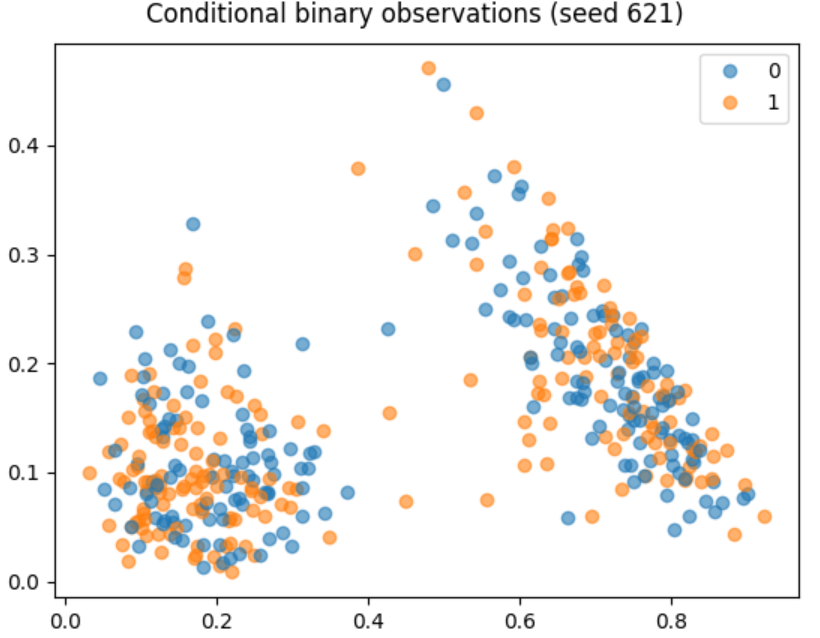
\includegraphics[scale=0.7]{images/samples_dirichlet_lc}
    \caption{Generated samples out of $K=2$ dirichlet distributions, labelized using the sigmoid modelisation on $\mathbb{P}(Y_i = 1)$.}
    \label{fig:dirichlet_lc_badconditioning}
\end{figure}

As previously, since the data lives in the simplex, they are too close to the border of the next label set, which ends up creating a blurry dataset for which the
linear model is not relevant anymore.